\chapter{Introduction}

\section{Overview}

The Global Arrays (GA) toolkit provides a shared memory style programming
environment in the context of distributed array data structures (called
``global arrays''). From the user perspective, a global array can be used as if
it was stored in shared memory. All details of the data distribution,
addressing, and data access are encapsulated in the global array objects.
Information about the actual data distribution and locality can be easily
obtained and taken advantage of whenever data locality is important. The
primary target architectures for which GA was developed are massively-parallel
distributed-memory and scalable shared-memory systems. 

GA divides logically shared data structures into ``local'' and ``remote''
portions. It recognizes variable data transfer costs required to access the
data depending on the proximity attributes. A local portion of the shared
memory is assumed to be faster to access and the remainder (remote portion) is
considered slower to access. These differences do not hinder the ease-of-use
since the library provides uniform access mechanisms for all the shared data
regardless where the referenced data is located. In addition, any processes can
access a local portion of the shared data directly/in-place like any other data
in process local memory. Access to other portions of the shared data must be
done through the GA library calls. 

GA was designed to complement rather than substitute the message-passing model,
and it allows the user to combine shared-memory and message-passing styles of
programming in the same program. GA inherits an execution environment from a
message-passing library (w.r.t. processes, file descriptors etc.) that started
the parallel program. 

GA is implemented as a library with C and Fortran-77 bindings, and there have
been also a Python and C++ interfaces (included starting with the release 3.2)
developed. Therefore, explicit library calls are required to use the GA model
in a parallel C/Fortran program. 

A disk extension of the Global Array library is supported by its companion
library called Disk Resident Arrays (DRA). DRA maintains array objects in
secondary storage and allows transfer of data to/from global arrays. 

\section{Basic Functionality}

The basic shared memory operations supported include \emph{get}, \emph{put},
\emph{scatter} and \emph{gather}. They are complemented by \emph{atomic}
\emph{read-and-increment}, \emph{accumulate} (reduction operation that combines
data in local memory with data in the shared memory location), and \emph{lock}
operations. However, these operations can only be used to access data in global
arrays rather than arbitrary memory locations. At least one global array has to
be created before data transfer operations can be used. These GA operations are
truly one-sided/unilateral and will complete regardless of actions taken by the
remote process(es) that own(s) the referenced data. In particular, GA does not
offer or rely on a polling operation or require inserting any other GA library
calls to assure communication progress on the remote side. 

A programmer in the GA program has a full control over the distribution of
global arrays. Both regular and irregular distributions are supported, see
Section 3 for details. 

The GA data transfer operations use an array index-based interface rather than
addresses of the shared data. Unlike other systems based on global address
space that support remote memory (\emph{put/get}) operations, GA does not
require the user to specify the target process/es where the referenced shared
data resides -- it simply provides a global view of the data structures. The
higher level array oriented API (application programming interface) makes GA
easier to use, at the same time without compromising data locality control. The
library internally performs global array index-to-address translation and then
transfers data between appropriate processes. If necessary, the programmer is
always able to inquire: 
\begin{itemize}
\item where an an element or array section is located, and 
\item which process or processes own data in the specified array section. 
\end{itemize}
The GA toolkit supports four data types in Fortran: integer, real, double
precision, and double complex. In the C interface, int, long, float, double and
struct double complex are available. Underneath, the library represents the
data using C datatypes. For the Fortran users, it means that some arrays
created in C for which there is no appropriate datatype mapping to Fortran (for
example on the Cray T3E Fortran real is not implemented whereas C float is)
might not be accessible.  In all the other cases, the dataype representation is
transparent. 

The supported array dimensions range from one to seven. This limit follows the
Fortran convention. The library can be reconfigured to support more than
7-dimensions but only through the C interface. 

\section{Programming Model}

The Global Arrays library supports two programming styles: task-parallel and
data-parallel. The GA task-parallel model of computations is based on the
explicit remote memory copy: The remote portion of shared data has to be copied
into the local memory area of a process before it can be used in computations
by that process. Of course, the ``local'' portion of shared data can always be
accessed directly thus avoiding the memory copy. 

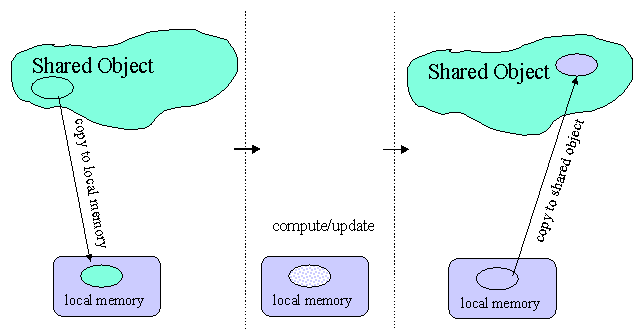
\includegraphics[width=4in]{mod}

The data distribution and locality control are provided to the programmer.  The
data locality information for the shared data is also available.  The library
offers a set of operations for management of its data structures, one-sided
data transfer operations, and supportive operations for data locality control
and queries. The GA shared memory consistency model is a result of a compromise
between the ease of use and a portable performance. The load and store
operations are guaranteed to be \emph{ordered} with respect to each other only
if they target overlapping memory locations. The store operations (\emph{put,
scatter}) and \emph{accumulate} complete locally before returning i.e., the
data in the user local buffer has been copied out but not necessarily completed
at the remote side. The memory consistency is only guaranteed for: 
\begin{itemize}
\item multiple read operations (as the data does not change), 
\item multiple accumulate operations (as addition is commutative), and 
\item multiple disjoint put operations (as there is only one writer for each
element). 
\end{itemize}
The application can manage consistency of its data structures in other cases by
using \emph{lock, barrier}, and \emph{fence} operations available in the
library. 

The data-parallel model is supported by a set of collective functions that
operate on global arrays or their portions. Underneath, if any interprocessor
communication is required, the library uses remote memory copy (most often) or
collective message-passing operations. 

\section{Application Guidelines}

These are some guidelines regarding suitability of the GA for different types
of applications. 

\subsection{When to use GA: }

Algorithmic Considerations 
\begin{itemize}
\item applications with dynamic and irregular communication patterns 
\item for calculations driven by dynamic load balancing 
\item need 1-sided access to shared data structures 
\item need high-level operations on distributed arrays and/or for out-of-core
array-based algorithms (GA + DRA) 
\end{itemize}
Useability Considerations
\begin{itemize}
\item data locality must be explicitly available 
\item when coding in message passing becomes too complicated 
\item when portable performance is important 
\item need object orientation without the overhead of C++ 
\end{itemize}

\subsection{When not to use GA}

Algorithmic Considerations 
\begin{itemize}
\item for systolic, or nearest neighbor communications with regular
communication patterns 
\item when synchronization associated with cooperative point-to-point message
passing is needed (e.g., Cholesky factorization in Scalapack) 
\end{itemize}
Usability Considerations 
\begin{itemize}
\item when interprocedural analysis and compiler parallelization is more
effective 
\item a parallel language support is sufficient and robust compilers available 
\end{itemize}
